% preambula dokumenta
\documentclass[a4paper, 10pt]{article}
\usepackage[slovene]{babel}
\usepackage[utf8]{inputenc}
\usepackage[T1]{fontenc}
\usepackage{lmodern}
\usepackage[pdftex]{graphics}
\usepackage{amsmath}
\usepackage{graphicx}
\usepackage{eurosym}
\usepackage{float}
\graphicspath{ {./images/} }

% telo dokumenta
\begin{document}
\title{Predpostavka o Randićevem indeksu in radiusu}
\author{Anja Žavbi Kunaver\\Jaka Munda}

\maketitle

\section{Opis problema}
Računalniški program Graffiti je postavil lemo, da za enostaven povezan graf $G=(V, E)$ velja, $$ Ra(G) \geq rad(G) -1$$

% Potrebno je testirati domnevo na različne načine na manjših in večjih grafih.
% Z uporabo metahevristične populacije je potrebno preizkusiti domnevo na večjih grafih in upati na njeno ovrgbo.

\subsection*{Opombe:}
\begin{enumerate}
\item Graf je enostaven, če ne vsebuje zank in je brez vzporednih povezav,
\item ekscentričnost vozlišča $v$ je razdalja do njegovega najbolj oddaljenega vozlišča; tj. $\max \{d(v,u) : u \in V(G) \}$,
%$rad(G)$ je radius grafa; tj. minimum ekscentričnosti vozlišč grafa.
\item radius grafa $rad(G)$ pa pomeni minimum ekscentričnosti vozlišč grafa,
\item
$Ra(G)$ je Randićev indeks grafa G. Definiran je kot
$$Ra(G) = \sum_{uv \in E(G)} \frac{1}{\sqrt{d(u) d(v)}},$$
\item $d(x)$ predstavlja stopnjo vozlišča $x$ oz. število povezav ki imajo vozlišče $x$ za svoje krajišče.
\end{enumerate}

%Računalniški program $Graffiti$ nam je postavil naslednjo lemo.

%Naj bo $G=(V,E)$ enostaven povezan graf, torej v grafu ni zank in ni vzporednih povezav. Potem velja neenakost: $$ Ra(G) \geq rad(G) -1$$ Tu smo z $Ra(G)$ označili randičev indeks, ki je %definiran kot: $$Ra(G) = \sum_{uv \in E(G)} \frac{1}{\sqrt{d(u) d(v)}},$$ kjer $d(x)$ predstavlja število povezav, ki imajo za svoje krajišče vozlišče $x$. Z $rad(G)$ pa smo označili radius %grafa $G$, kar pomeni najmansa najvecja razdalja med dvema vozliščema.

\section{Opis dela}

Lemo bova testirala v sagu. Sprva na malih grafih in sicer bova sprogramirala funkcijo ki bo preverila ali drži neenakost na vseh enostavnih malih grafih z $n$ vozlišči. Če bo lema držala na vseh manjših grafih, bova z uporabo populacijske metahevristike poskušala ovreči to neenakost na velikih grafih.

\section{Primer}

\begin{align*}
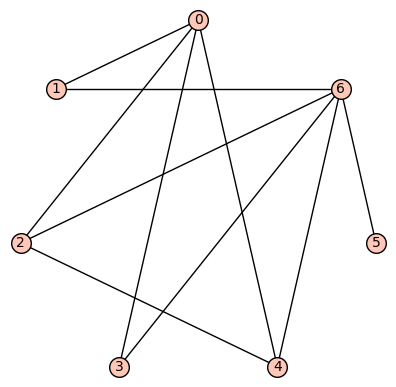
\includegraphics{primer}
\end{align*}

$$radius = 2$$
$$Randičev \ indeks \doteq 2.47$$
$$2.47 > 2 - 1$$

Vidimo da na tem grafu lema drži.



\end{document}